\documentclass[12pt, a4paper]{article}
\usepackage[utf8]{inputenc}
\usepackage[spanish]{babel}
\usepackage{amsmath}
\usepackage{graphicx}
\usepackage{geometry}
\usepackage{caption}
\usepackage{cite}

\geometry{a4paper, margin=1in}
\linespread{1.5}

\title{Análisis Comparativo de la Sincronización en Redes Complejas: \\ El Modelo de Kuramoto en Topologías Homogéneas y Libres de Escala}
\author{Gaspar Dip}
\date{\today}

\begin{document}

\maketitle

\begin{abstract}
\noindent La sincronización es un fenómeno de orden colectivo omnipresente en sistemas naturales y artificiales. El modelo de Kuramoto ofrece un marco matemático canónico para estudiar la transición del desorden a la coherencia en poblaciones de osciladores acoplados. Este trabajo extiende el modelo clásico, que asume un acoplamiento global, para investigar cómo la topología de la red subyacente influye en la dinámica de la sincronización. Se realiza un análisis computacional comparativo entre dos arquetipos de red: el grafo completo, como modelo de una red homogénea, y la red libre de escala generada por el modelo de Barabási-Albert, como representante de redes heterogéneas con hubs. Mediante simulaciones a gran escala (\(N=10000\)) aceleradas por GPU, se demuestra que la topología dicta fundamentalmente la naturaleza de la transición de fase. Se observa que, si bien las redes libres de escala presentan un umbral de acoplamiento crítico (\(K_c\)) más alto, su transición es más gradual y está mediada por un mecanismo jerárquico iniciado en los hubs. Finalmente, se presenta un análisis estadístico del \(K_c\) y una visualización detallada que revela la compleja interacción entre la centralidad estructural (grado) y el comportamiento dinámico (frecuencia efectiva) de los nodos.
\end{abstract}

\newpage

\section{Introducción}

El surgimiento espontáneo del orden a partir de interacciones locales es uno de los conceptos más fascinantes de la ciencia de la complejidad. Fenómenos como el parpadeo al unísono de las luciérnagas, la activación coordinada de neuronas en el cerebro o la sincronía de los aplausos en una audiencia, son manifestaciones de un principio universal de autoorganización \cite{Strogatz2003}.

El modelo de Kuramoto, propuesto por Yoshiki Kuramoto en 1975, se ha establecido como el paradigma matemático para el estudio de estos fenómenos \cite{Kuramoto1975}. En su forma original, describe una población de osciladores donde cada uno influye en todos los demás de manera uniforme (acoplamiento de campo medio o "all-to-all"). Sin embargo, la mayoría de los sistemas del mundo real no presentan esta conectividad total. Las interacciones están restringidas a una estructura de red compleja, a menudo con propiedades no triviales.

Este trabajo aborda la pregunta fundamental: ¿cómo afecta la topología de la red al proceso de sincronización? Para ello, se implementa el modelo de Kuramoto sobre dos tipos de redes diametralmente opuestas:
\begin{itemize}
    \item \textbf{El Grafo Completo:} Una red homogénea y "democrática", donde cada nodo tiene la misma importancia estructural. Sirve como nuestra línea de base, equivalente al modelo original de Kuramoto.
    \item \textbf{La Red Libre de Escala:} Una red heterogénea y "jerárquica", caracterizada por la presencia de unos pocos nodos altamente conectados (hubs) y una gran mayoría de nodos con pocas conexiones. Este modelo, generado por el algoritmo de Barabási-Albert \cite{Barabasi1999}, describe con gran precisión la estructura de muchas redes reales, como Internet o las redes sociales.
\end{itemize}

A través de simulaciones numéricas a gran escala, se investigará la transición de fase del desorden a la sincronización, se visualizarán los mecanismos subyacentes y se cuantificará la robustez de los resultados.

\section{Metodología}

\subsection{El Modelo de Kuramoto en Redes}

La dinámica de la fase \(\theta_i\) de cada uno de los \(N\) osciladores en la red se rige por la siguiente ecuación diferencial:
$$
\frac{d\theta_i}{dt} = \omega_i + \frac{K}{k_i} \sum_{j=1}^{N} A_{ij} \sin(\theta_j - \theta_i)
$$
donde:
\begin{itemize}
    \item \(\omega_i\) es la frecuencia natural del oscilador \(i\), extraída de una distribución Gaussiana \(N(\mu, \sigma^2)\). En este trabajo, se utiliza \(\mu=0\) y \(\sigma=0.5\).
    \item \(K\) es la constante de acoplamiento global, que modula la fuerza de la interacción.
    \item \(k_i = \sum_j A_{ij}\) es el grado del nodo \(i\). La normalización por \(k_i\) asegura que la influencia total que recibe un nodo no dependa trivialmente de su número de conexiones.
    \item \(A_{ij}\) es el elemento \((i, j)\) de la matriz de adyacencia de la red, siendo 1 si los nodos \(i\) y \(j\) están conectados y 0 en caso contrario.
\end{itemize}

Computacionalmente, el término de la suma \(\sum_j A_{ij} \sin(\theta_j - \theta_i)\) presenta un desafío para redes grandes. Un cálculo directo requeriría la construcción de una matriz de diferencias de fase de tamaño \(N \times N\), lo cual es inviable en memoria para \(N > 10^4\). Para superar esto, se utiliza la identidad trigonométrica \(\sin(\theta_j - \theta_i) = \sin(\theta_j)\cos(\theta_i) - \cos(\theta_j)\sin(\theta_i)\). Esto permite reescribir el término de interacción de forma que solo requiere multiplicaciones de la matriz de adyacencia dispersa por vectores, reduciendo el consumo de memoria de \(O(N^2)\) a \(O(E)\), donde \(E\) es el número de aristas.

\subsection{Simulación Numérica}

Las simulaciones se implementaron en Python utilizando la librería \texttt{CuPy} para realizar los cálculos en una GPU, permitiendo analizar redes de hasta \(N=10000\) nodos. El sistema de ecuaciones diferenciales se resolvió numéricamente mediante un integrador de Euler de primer orden con un paso de tiempo fijo (\(DT=0.01\)).

Para asegurar que las mediciones se realizan en el estado estacionario del sistema, cada simulación se dividió en dos fases:
\begin{itemize}
  \item \textbf{Fase Transitoria (\(T_{\text{transient}}\)):} Un período inicial durante el cual el sistema evoluciona para alcanzar un estado de equilibrio dinámico. Los datos de esta fase se descartan.
  \item \textbf{Fase de Medición (\(T_{\text{measure}}\)):} Un período posterior durante el cual se calcula el parámetro de orden en múltiples puntos para obtener un valor promedio robusto, mitigando el efecto de las fluctuaciones.
\end{itemize}

\subsection{Métricas de Análisis}

\begin{itemize}
    \item \textbf{Parámetro de Orden Global (r):} Para cuantificar el nivel de sincronización global, se utiliza el parámetro de orden de Kuramoto:
    $$
    r(t) = \left| \frac{1}{N} \sum_{j=1}^{N} e^{i\theta_j(t)} \right|
    $$
    Un valor de \(r \approx 0\) indica un estado desordenado, mientras que \(r \approx 1\) representa una sincronización perfecta.

    \item \textbf{Umbral Crítico (Kc):} Se define como el valor de \(K\) para el cual el parámetro de orden en estado estacionario, \(r_{\infty}\), cruza por primera vez un umbral predefinido (en este caso, \(r > 0.5\)).

    \item \textbf{Frecuencia Efectiva (\(\Omega_i\)):} Se calcula como la velocidad de cambio promedio de la fase de un oscilador en la segunda mitad de la simulación. Mide la velocidad de rotación real del oscilador en el estado estacionario.
\end{itemize}

\section{Resultados}

\subsection{Transición a la Sincronización Global}

Para comparar el comportamiento macroscópico de ambas topologías, se realizó un barrido del parámetro de acoplamiento \(K\) para redes de \(N=10000\) nodos. La Figura \ref{fig:r_vs_k} muestra la transición del parámetro de orden \(r\).

\begin{figure}[h!]
    \centering
    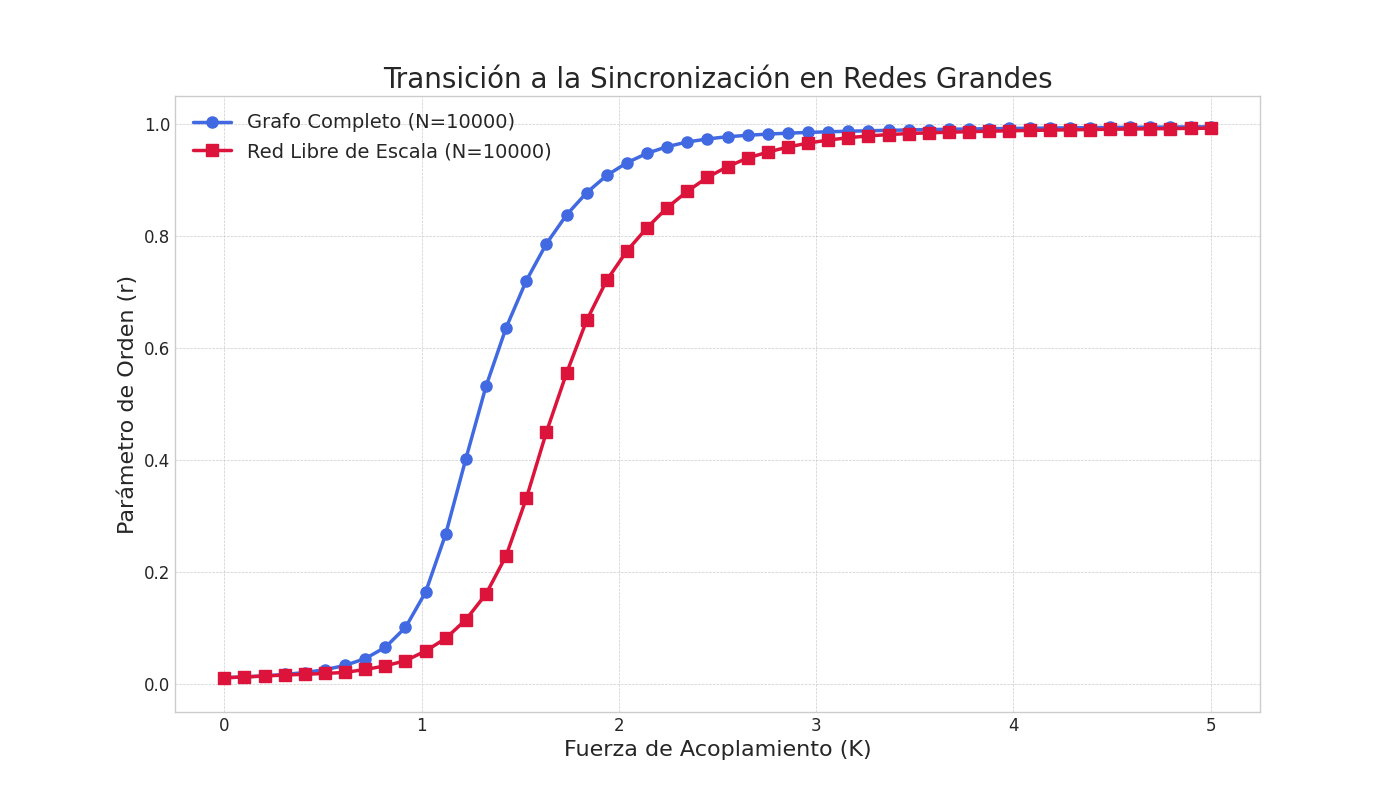
\includegraphics[width=\textwidth]{./img/1.png}
    \caption{Parámetro de orden \(r\) en función de la fuerza de acoplamiento \(K\) para un Grafo Completo (azul) y una Red Libre de Escala (rojo) con \(N=10000\) nodos. Se observa que el grafo completo presenta una transición más abrupta y a un \(K_c\) menor que la red libre de escala.}
    \label{fig:r_vs_k}
\end{figure}

\subsection{Análisis Visual de la Dinámica en Redes Libres de Escala}

Para entender el mecanismo subyacente a la transición gradual, se visualizó el estado de la red en tres regímenes clave, definidos en relación a su \(K_c\) calculado. Para mejorar la claridad, las visualizaciones se centran en el "esqueleto" de la red, mostrando únicamente los nodos con un grado superior a un umbral. En la Figura \ref{fig:visual_states}, el tamaño de cada nodo es proporcional a su grado y su color representa su fase.

\begin{figure}[h!]
    \centering
    % ####################################################################
    % ACCIÓN REQUERIDA:
    % Inserta aquí los tres gráficos generados por el Script Final (V5).
    % Puedes unirlos en una sola imagen o insertarlos por separado.
    % Guarda la imagen como "visual_states.png".
    % ####################################################################
    \includegraphics[width=\textwidth]{visual_states.png}
    \caption{Visualización de la red libre de escala en tres estados: Desordenado (izquierda, \(K < K_c\)), Sincronización Parcial (centro, \(K \approx K_c\)) y Sincronización Fuerte (derecha, \(K >> K_c\)). El color representa la frecuencia efectiva (blanco \(\approx 0\), rojo/azul \(\neq 0\)).}
    \label{fig:visual_states}
\end{figure}

\subsection{Análisis Estadístico del Umbral Crítico}

Dado el carácter aleatorio del modelo de Barabási-Albert, se realizó un análisis estadístico para caracterizar la distribución del umbral crítico \(K_c\). Se ejecutaron 1000 simulaciones independientes con redes de \(N=10000\).

% ####################################################################
% ACCIÓN REQUERIDA:
% Ejecuta el Script 4 y rellena los siguientes valores.
% Inserta el histograma generado.
% ####################################################################
El valor promedio (esperanza) de \(K_c\) fue de \textbf{[INSERTAR MEDIA AQUÍ]}, con una desviación estándar de \textbf{[INSERTAR DESVIACIÓN ESTÁNDAR AQUÍ]}. La distribución de los valores se muestra en la Figura \ref{fig:kc_hist}.

\begin{figure}[h!]
    \centering
    \includegraphics[width=0.7\textwidth]{kc_hist.png}
    \caption{Histograma de la distribución de los valores del umbral crítico \(K_c\) obtenidos a partir de 1000 realizaciones de redes libres de escala con \(N=10000\).}
    \label{fig:kc_hist}
\end{figure}

\section{Discusión y Conclusiones}

Los resultados presentados revelan una profunda influencia de la topología de la red en la dinámica de la sincronización.

El análisis comparativo (Figura \ref{fig:r_vs_k}) muestra que, si bien el grafo completo se sincroniza a un umbral de acoplamiento menor, su transición es extremadamente abrupta. Esto sugiere un fenómeno de "todo o nada" característico de los sistemas homogéneos. Por el contrario, la red libre de escala exhibe una transición más suave y gradual, lo que apunta a un mecanismo de sincronización jerárquico.

La visualización de los estados dinámicos (Figura \ref{fig:visual_states}) confirma esta hipótesis. En el régimen de sincronización parcial, se observa claramente la formación de un núcleo de osciladores sincronizados (nodos de color pálido) que coexiste con una periferia de osciladores "a la deriva" (nodos de colores intensos). Es crucial notar que los nodos más grandes (hubs) no son necesariamente los más perfectamente sincronizados (no son los más blancos), lo que sugiere una compleja interacción entre la centralidad estructural y las propiedades dinámicas intrínsecas de cada nodo.

Finalmente, el análisis estadístico (Figura \ref{fig:kc_hist}) demuestra la robustez de estos hallazgos. La baja desviación estándar del \(K_c\) indica que el comportamiento de sincronización es una propiedad característica de la clase de redes libres de escala, y no un artefacto de una única realización aleatoria.

En conclusión, este trabajo demuestra que la estructura heterogénea de las redes libres de escala da lugar a un mecanismo de sincronización jerárquico, iniciado por los hubs pero perfeccionado por los nodos más "dóciles", que es fundamentalmente diferente de la transición abrupta y colectiva observada en redes homogéneas.

\begin{thebibliography}{9}
\bibitem{Strogatz2003}
Strogatz, S. H. (2003). \textit{Sync: The emerging science of spontaneous order}. Hyperion.

\bibitem{Kuramoto1975}
Kuramoto, Y. (1975). Self-entrainment of a population of coupled non-linear oscillators. In \textit{International Symposium on Mathematical Problems in Theoretical Physics} (pp. 420-422). Springer, Berlin, Heidelberg.

\bibitem{Barabasi1999}
Barabási, A. L., \& Albert, R. (1999). Emergence of scaling in random networks. \textit{Science}, 286(5439), 509-512.
\end{thebibliography}

\end{document}